\section{Fees and Rewards}\label{sec:tokenomics}

Taiko users pay Ether (ETH) as their transaction fees; block \emph{proposers} receive all the transaction fees in every block they successfully propose and in return, they need to burn a certain amount of Taiko Token (TKO) to propose the blocks to the protocol and pay Ether to Ethereum validators for their block proposals to be included in L1 blocks. When L2 blocks are verified by block \emph{provers}, the protocol mints additional TKO tokens to reward the proofs. The TKO token is transparent to L2 users, which allows the same user experience as on the Ethereum chain.

\begin{Figure}
 \centering
 % \includegraphics[width=\linewidth]{fig/taikoEcosystem.png}
 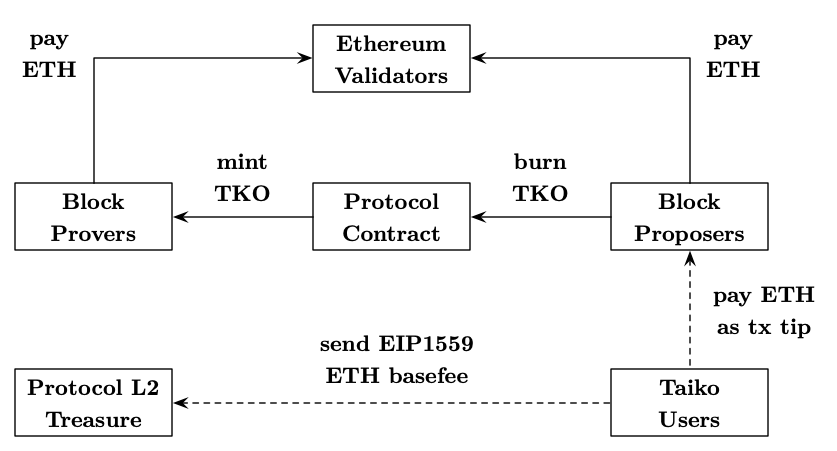
\includegraphics[width=\linewidth]{fig/fees_and_rewards.png}
 \captionof{figure}{The flow of payments, fees and rewards.}
 \label{fig:taiExchange}

\end{Figure}


\subsection{Motivation}
We design price dynamics that evolve with respect to a number of different factors (without the use of any price oracles):
\begin{enumerate}
\item The L2 block space. Although block space is much cheaper than on L1, it is still necessary to adjust its price in a way to avoid L2 space being abused. We will enable EIP-1559 on Taiko L2 to dynamically adjust the block space price in a later release (see Section \ref{sec:eip1559-propose}).
\item Protection against external factors, such as TKO token price fluctuations and competing L2 solutions, that can deter proposer and prover engagement with the protocol. Our design enables a dynamic system that introduces fee discounts and reward premiums as incentives, when current engagement falls below average proposal/proof delay statistics.

\item The current number of unverified blocks. The Taiko protocol has a fixed number of slots, $n_\textnormal{slot}$, for block proposals to allow for parallel proof computation. When there are more unverified blocks occupying the available slots, fees (and rewards) will increase to adjust for the competition within the group of proposers (and similarly for provers).
% (MEV: REMOVED THIS PART BUT HAPPY TO DISCUSS AND INCLUDE WHAT THIS IS TRYING TO SAY.)
% % prevent slots from being over-sold
% -- this is due to the asynchronous nature of proposals and proofs, therefore, the adjustment of fees and rewards doesn't happen after each block proposal or proof.

\item A system that benefits early adopters, working as base discounts for proposal fees that diminish over time, as proposers may be more vulnerable at the initial stages of the protocol compared to provers.
\end{enumerate}

% Our overall fees for proposers and rewards for provers will be a summation of these four components. In this section, we will focus on the last three building blocks.

At the time of submission of a proposal or a proof, referred to as $t$, a proposal fee $f(t)$ or a proof reward $r(t)$ respectively, is calculated as a product of a \textit{base fee} $f_\textnormal{base}$, time-based \emph{incentive multipliers}, $\alpha^+(t)$ and $\alpha^-(t)$, and \emph{slot-availability multipliers}, $\beta^+(n)$ and $\beta^-(n)$, that are based on the number of unverified blocks $n$.
% \begin{align}
% f(t) = f_\textnormal{base} \cdot \beta_\textnormal{icv}^+ \cdot \beta_\textnormal{slot}^+
% \\
% r(t) = f_\textnormal{base} \cdot \beta_\textnormal{icv}^- \cdot \beta_\textnormal{slot}^-
% \end{align}
\begin{align}
f(t) = f_\textnormal{base} \cdot \alpha^+(t) \cdot \beta^+(n)
\\
r(t) = f_\textnormal{base}
\cdot \alpha^-(t) \cdot \beta^-(n)
\end{align}

Although $t$ is determined from the moment of submission of a proof, similar to a proposal, the actual moment of issuing the reward to a prover is potentially much later, when the proof is validated through a series of other proofs that connect it to the genesis block. In other words, proof rewards are determined at the time of submission and minted at the time of validation.

Throughout the rest of the section, we will use the superscript $^+$ for constants, variables and functions specific to proposals (which add new unverified blocks) and $^-$ for constants, variables and functions specific to proofs (which remove unverified blocks).

% \subsection{Base Fee}
% The Taiko protocol maintains an internal state variable $f_\textnormal{base}$ called the \textit{Base Fee}.

% The $f(t)$ dynamics incorporates time based incentives by not discarding them after they are applied but using them to update $f_\textnormal{base}$ through averaging.
% \subsection{Constants}
% Taiko protocol maintains a number of internal constants $(n, f_\textnormal{base}, t_\textnormal{avg}, t_\textnormal{last})$

\subsection{State Variables}
Taiko protocol maintains a number of internal state variables $(n, f_\textnormal{base}, t^+_\textnormal{ave}, t^-_\textnormal{ave}, t^+_\textnormal{last}, t^-_\textnormal{last})$ that get updated after every successful block proposal or validated proof.
\begin{itemize}
    \item $n$ is the current number of unverified blocks. Initially, $n$ is set to $0$.
    \item $f_\textnormal{base}$ is the base fee, computed as a moving average of its product with incentive multipliers. Initially $f_\textnormal{base}$ is set to a constant $f_\textnormal{init}$.
    \item $t^+_\textnormal{ave}$ is the average duration between proposal submissions conditioned on that they are successful. Initially, $t^+_\textnormal{ave}$ is set to $K_\textnormal{max}^+$.
    % , computed as a moving average of the gap between the current successful submission and the previous successful submission.
    \item $t^-_\textnormal{ave}$ is the average duration between proof submissions conditioned on that they are eventually validated. Initially, $t^+_\textnormal{ave}$ is set to $K_\textnormal{max}^-$.
    % , computed as a moving average of the gap between the current validated submission and the previous validated submission.
    \item $t^+_\textnormal{last}$ is the submission time of the last successful proposal. Initially $t^+_\textnormal{last}$ is set to $0$.
    \item $t^-_\textnormal{last}$ is the submission time of the last validated proof. Initially $t^-_\textnormal{last}$ is set to $0$.
\end{itemize}
We discuss the state update at the end of the section, after discussing fee and reward computations in a particular state (see Section \ref{sec:priceStateUpdate}).




% \subsection{Time variables}
% Variables of time are a tuple of three elements: $(t, t_\textnormal{last}, t_\textnormal{ave})$.
% \begin{itemize}

%     \item $t_\textnormal{ave}$ is the average duration between proposals or proofs, computed as a moving average of the gap between $t$ and $t_\textnormal{last}$.
% \end{itemize}


\subsection{Incentive Multipliers}
\label{sec:incentive_mult}
Given a constant $K_\textnormal{inc} > 1$,
$\alpha^+(t): \mathbb{R}^+\rightarrow [ \nicefrac{1}{K_\textnormal{inc}},1]$ and $\alpha^-(t): \mathbb{R}^+\rightarrow [1, K_\textnormal{inc}] $ are time sensitive multipliers that can decrease fees and increase rewards.

Their purpose is to incentivize (to a certain degree) proposals and proofs when there are unpredictable deterrents acting against the engagement of proposers or provers, such as imbalances in the pricing that favor one side of the protocol at the expense of the other (internal);  competing L2 marketplaces that offer better deals at the moment or price fluctuations of the TKO token (external).

Incentive multipliers can gradually change the state variable $f_\textnormal{base}$, as will be explained in Section \ref{sec:priceStateUpdate}.

% In order to simplify exposition, in the rest of this section, we drop the superscripts of $t^\textnormal{prop}_\textnormal{ave}, t^\textnormal{proof}_\textnormal{ave}, t^\textnormal{prop}_\textnormal{last}, t^\textnormal{proof}_\textnormal{last}$ and refer to them as $t_\textnormal{ave}, t_\textnormal{last}$ depending on the context, i.e. when computing $\alpha_f(t)$, $t_\textnormal{ave}, t_\textnormal{last}$ will refer to $t^\textnormal{prop}_\textnormal{ave}, t^\textnormal{prop}_\textnormal{last}$ respectively; and when computing $\alpha_r(t)$, $t_\textnormal{ave}, t_\textnormal{last}$ will refer to $t^\textnormal{proof}_\textnormal{ave}, t^\textnormal{proof}_\textnormal{last}$ respectively.
\subsubsection{Intermediate Time Variables}
\label{sec:intermediateTimeVar}
% Time-based incentives begin when there is not any successful proposals or proofs for a period longer than
% a multiple of either; (1) the average duration between proposals or proofs, (2) $T_\textnormal{prop}$ for proposals or $T_\textnormal{proof}$ for proofs.

Given constants $K_\textnormal{grace} \geq 0$,
$K_\textnormal{activation} > 0$, $K^+_\textnormal{max}>0$, $K^-_\textnormal{max}>0$ and state variables, we can compute the following intermediate time variables, $t_\textnormal{grace}$ and $t_\textnormal{activation}$:
\begin{align}
t^+_\textnormal{grace} &\equiv
 K_\textnormal{grace} \cdot \min(t^+_\textnormal{ave}, K^+_\textnormal{max})\\
t^-_\textnormal{grace} &\equiv K_\textnormal{grace} \cdot \min(t^-_\textnormal{ave}, K^-_\textnormal{max}).
\end{align}
% \begin{align}
%     t_\textnormal{grace} \equiv
%  \begin{dcases}
%  K_\textnormal{grace} \cdot \min(t^+_\textnormal{ave}, K^+_\textnormal{max}), &\text{if a \emph{proposal}} \\
% K_\textnormal{grace} \cdot \min(t^-_\textnormal{ave}, K^-_\textnormal{max}), &\text{if a \emph{proof}}
% \end{dcases}
% \end{align}
% or, omitting the superscripts,
% \begin{align}
%     t_\textnormal{grace} \equiv
%  K_\textnormal{grace} \cdot \min(t_\textnormal{ave}, K_\textnormal{max}).
% \end{align}
% \begin{align}
% t_\textnormal{grace}  \equiv  K_\textnormal{GracePeriod} \cdot \min(t^\textnormal{proof}_\textnormal{ave}, K_\textnormal{BlockTimeCap})
% \end{align}
$t_\textnormal{grace}$ is the grace period starting at $t_\textnormal{last}$ (omitting the superscript) in which there are no incentives yet.
% do not activate and $f_\textnormal{min}$ remains unchanged. It is related to $t_\textnormal{ave}$ through $t_\textnormal{grace} = k_{\textnormal{grace}} \cdot t_\textnormal{ave}$.
% \begin{align}
%     t_\textnormal{max} \equiv
%  \begin{dcases}
%  K_\textnormal{max} \cdot \min(t^\textnormal{prop}_\textnormal{ave}, T_\textnormal{prop}), &\text{if a \emph{proposal}} \\
% K_\textnormal{max} \cdot \min(t^\textnormal{proof}_\textnormal{ave}, T_\textnormal{proof}), &\text{if a \emph{proof}}
% \end{dcases}
% \end{align}
% \begin{align}
% t_\textnormal{activation} \equiv
%  K_\textnormal{activation} \cdot \min(t_\textnormal{ave}, K_\textnormal{max}).
% \end{align}
\begin{align}
t^+_\textnormal{activation} &\equiv
 K_\textnormal{activation} \cdot \min(t^+_\textnormal{ave}, K^+_\textnormal{max})\\
t^-_\textnormal{activation} &\equiv
 K_\textnormal{activation} \cdot \min(t^-_\textnormal{ave}, K^-_\textnormal{max}).
\end{align}
% \begin{align}
% t_\textnormal{max}  \equiv   K_{\mathrm{MaxPeriod}} \cdot \min(t_\textnormal{ave}, K_\textnormal{ProofTimeCap})
% \end{align}

$t_\textnormal{activation}$ is the time period after which incentives reach their maximum effects from the time they first start to take effect at $t_\textnormal{last}+t_\textnormal{grace}$ (omitting the superscripts).
\begin{Figure}
 \centering
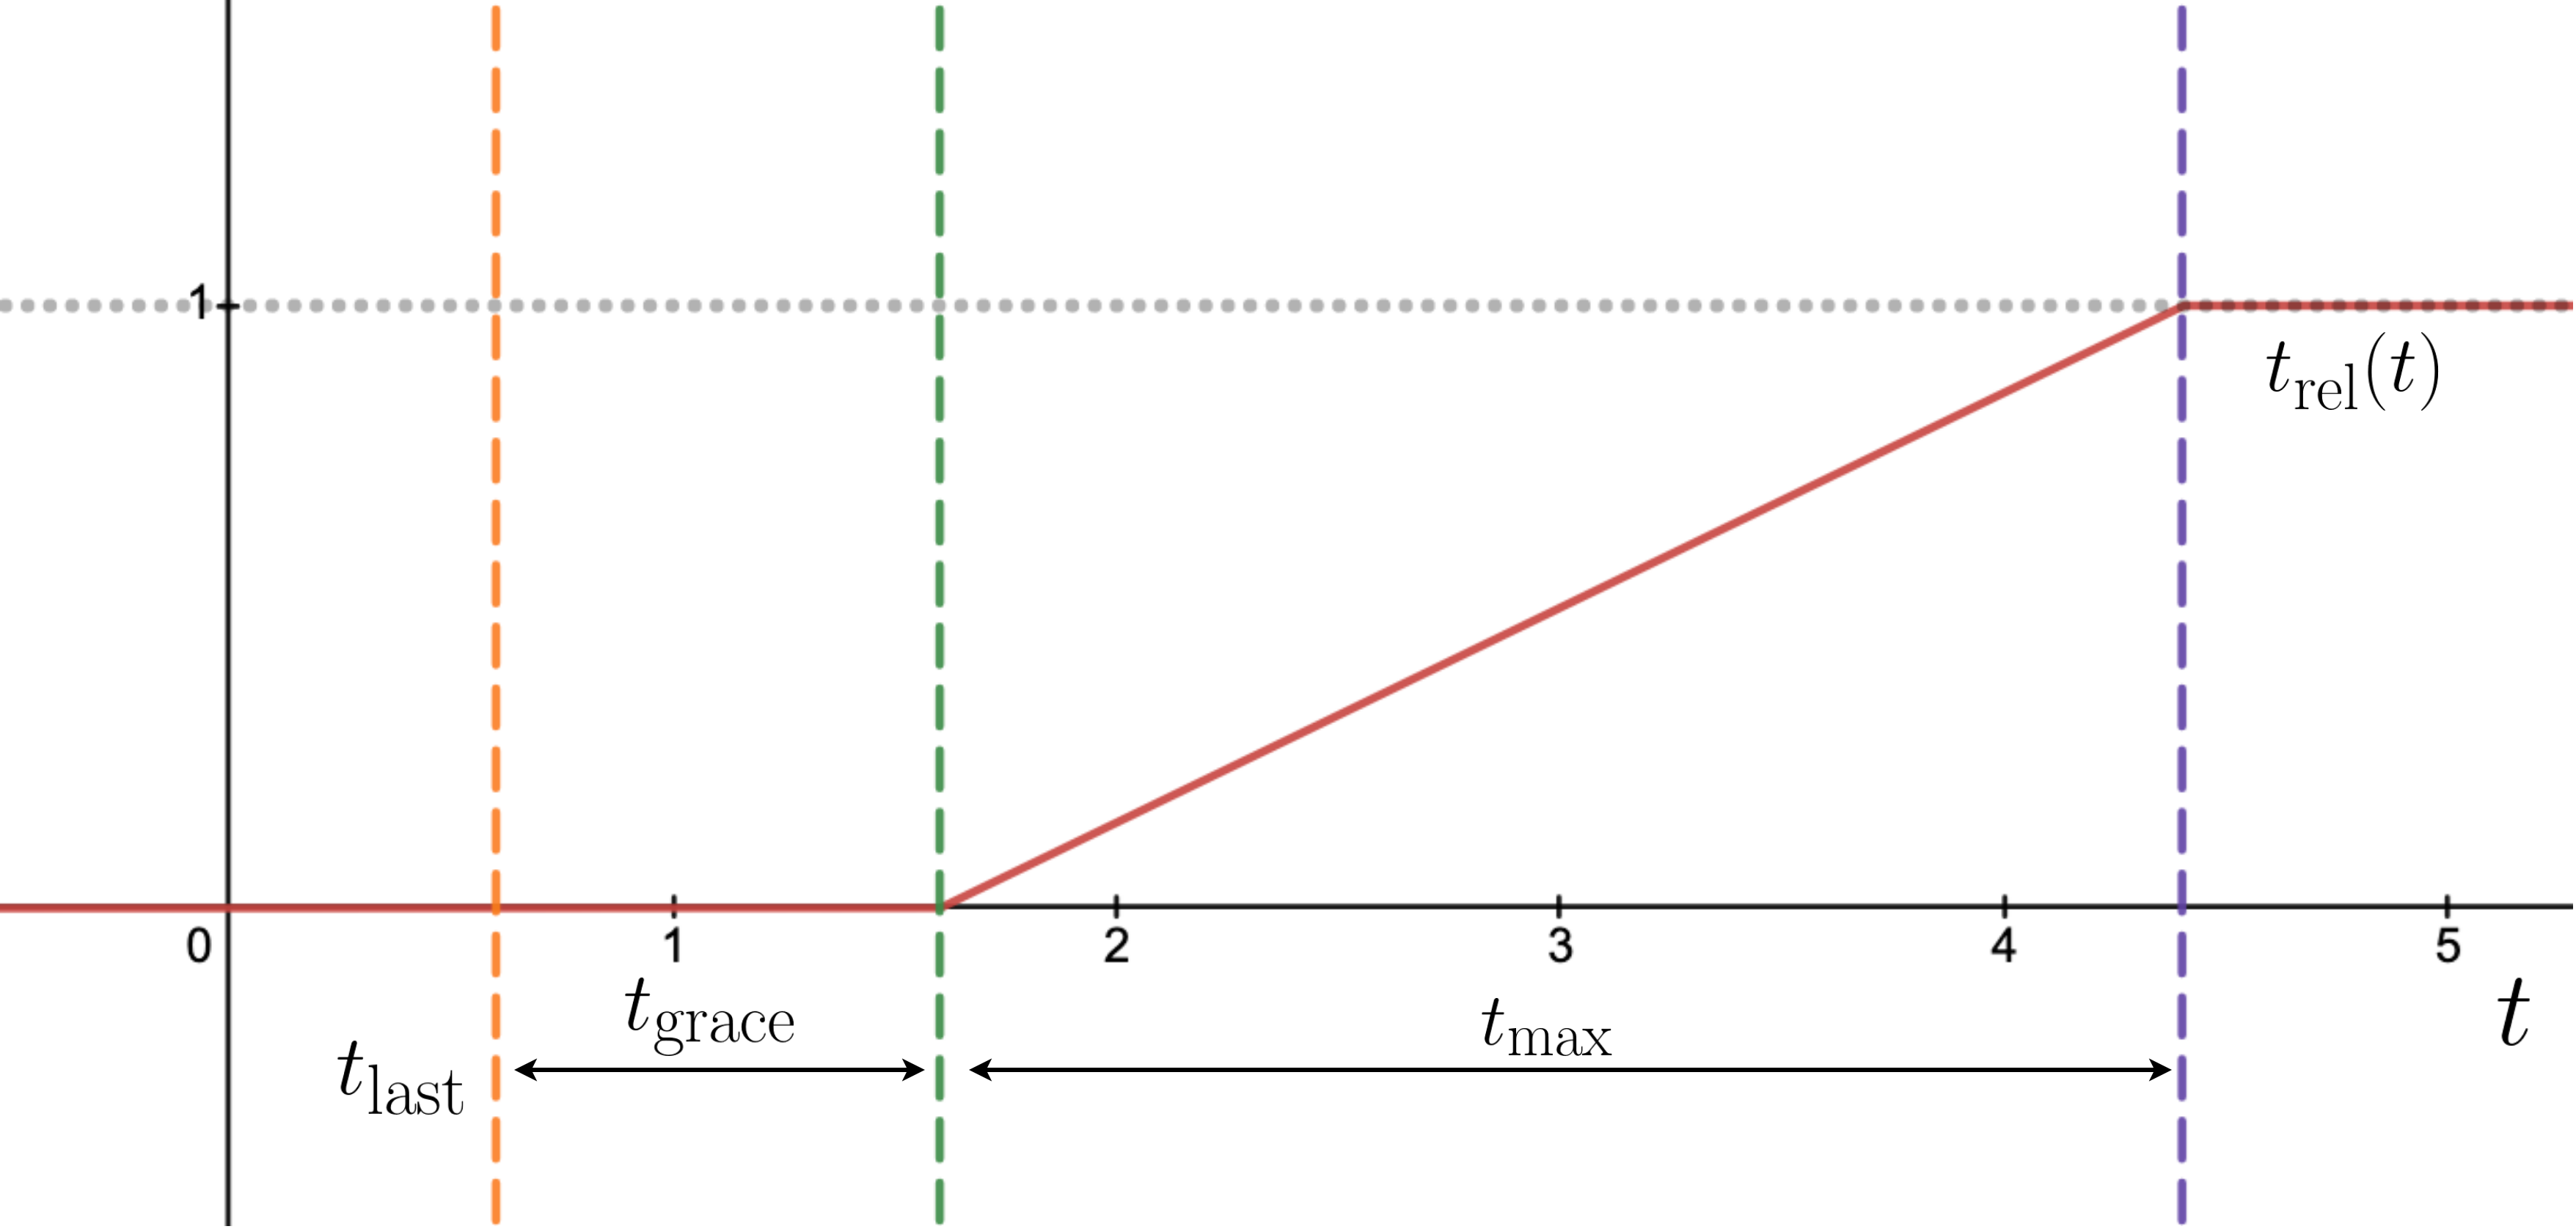
\includegraphics[width=0.9\linewidth]{fig/relative_time_graph.png}
 % \vspace{-0.2in}
 \vspace{-0.1in}
 \captionof{figure}{The graph of $t_\textnormal{rel}$ (red) with respect to time $t$ given $t_\textnormal{last}$, $t_\textnormal{grace}$, $t_\textnormal{activation}$ (omitting the superscripts).}
\label{fig:relativetime}
\end{Figure}

Two functions of note are $t^+_\textnormal{rel}(t),t^-_\textnormal{rel}(t): \mathbb{R}^+ \rightarrow [0,1]$ and they are defined as
\begin{align}
t_\textnormal{rel}^+(t) &=
% \frac{\textnormal{min}(\textnormal{max}(0, t - (t_{\textnormal{last}} + t_{\textnormal{grace}})), t_{\textnormal{max}})}{t_{\textnormal{max}}}
\textnormal{min}\left(\textnormal{max}\left(0, \frac{t - (t^+_\textnormal{last} + t^+_\textnormal{grace})}{t^+_\textnormal{activation}}\right), 1\right)\\
t_\textnormal{rel}^-(t) &=
% \frac{\textnormal{min}(\textnormal{max}(0, t - (t_{\textnormal{last}} + t_{\textnormal{grace}})), t_{\textnormal{max}})}{t_{\textnormal{max}}}
\textnormal{min}\left(\textnormal{max}\left(0, \frac{t - (t^-_\textnormal{last} + t^-_\textnormal{grace})}{t^-_\textnormal{activation}}\right), 1\right)
.
\end{align}

$t_\textnormal{rel}$ indicates \emph{relative normalized time}, and determines the activation point of time-based incentives, where $t_\textnormal{rel}$ becomes greater than $0$, and the saturation point of incentives, where $t_\textnormal{rel}$ becomes equal to $1$ (see Figure \ref{fig:relativetime}).

\begin{Figure}
 \centering
 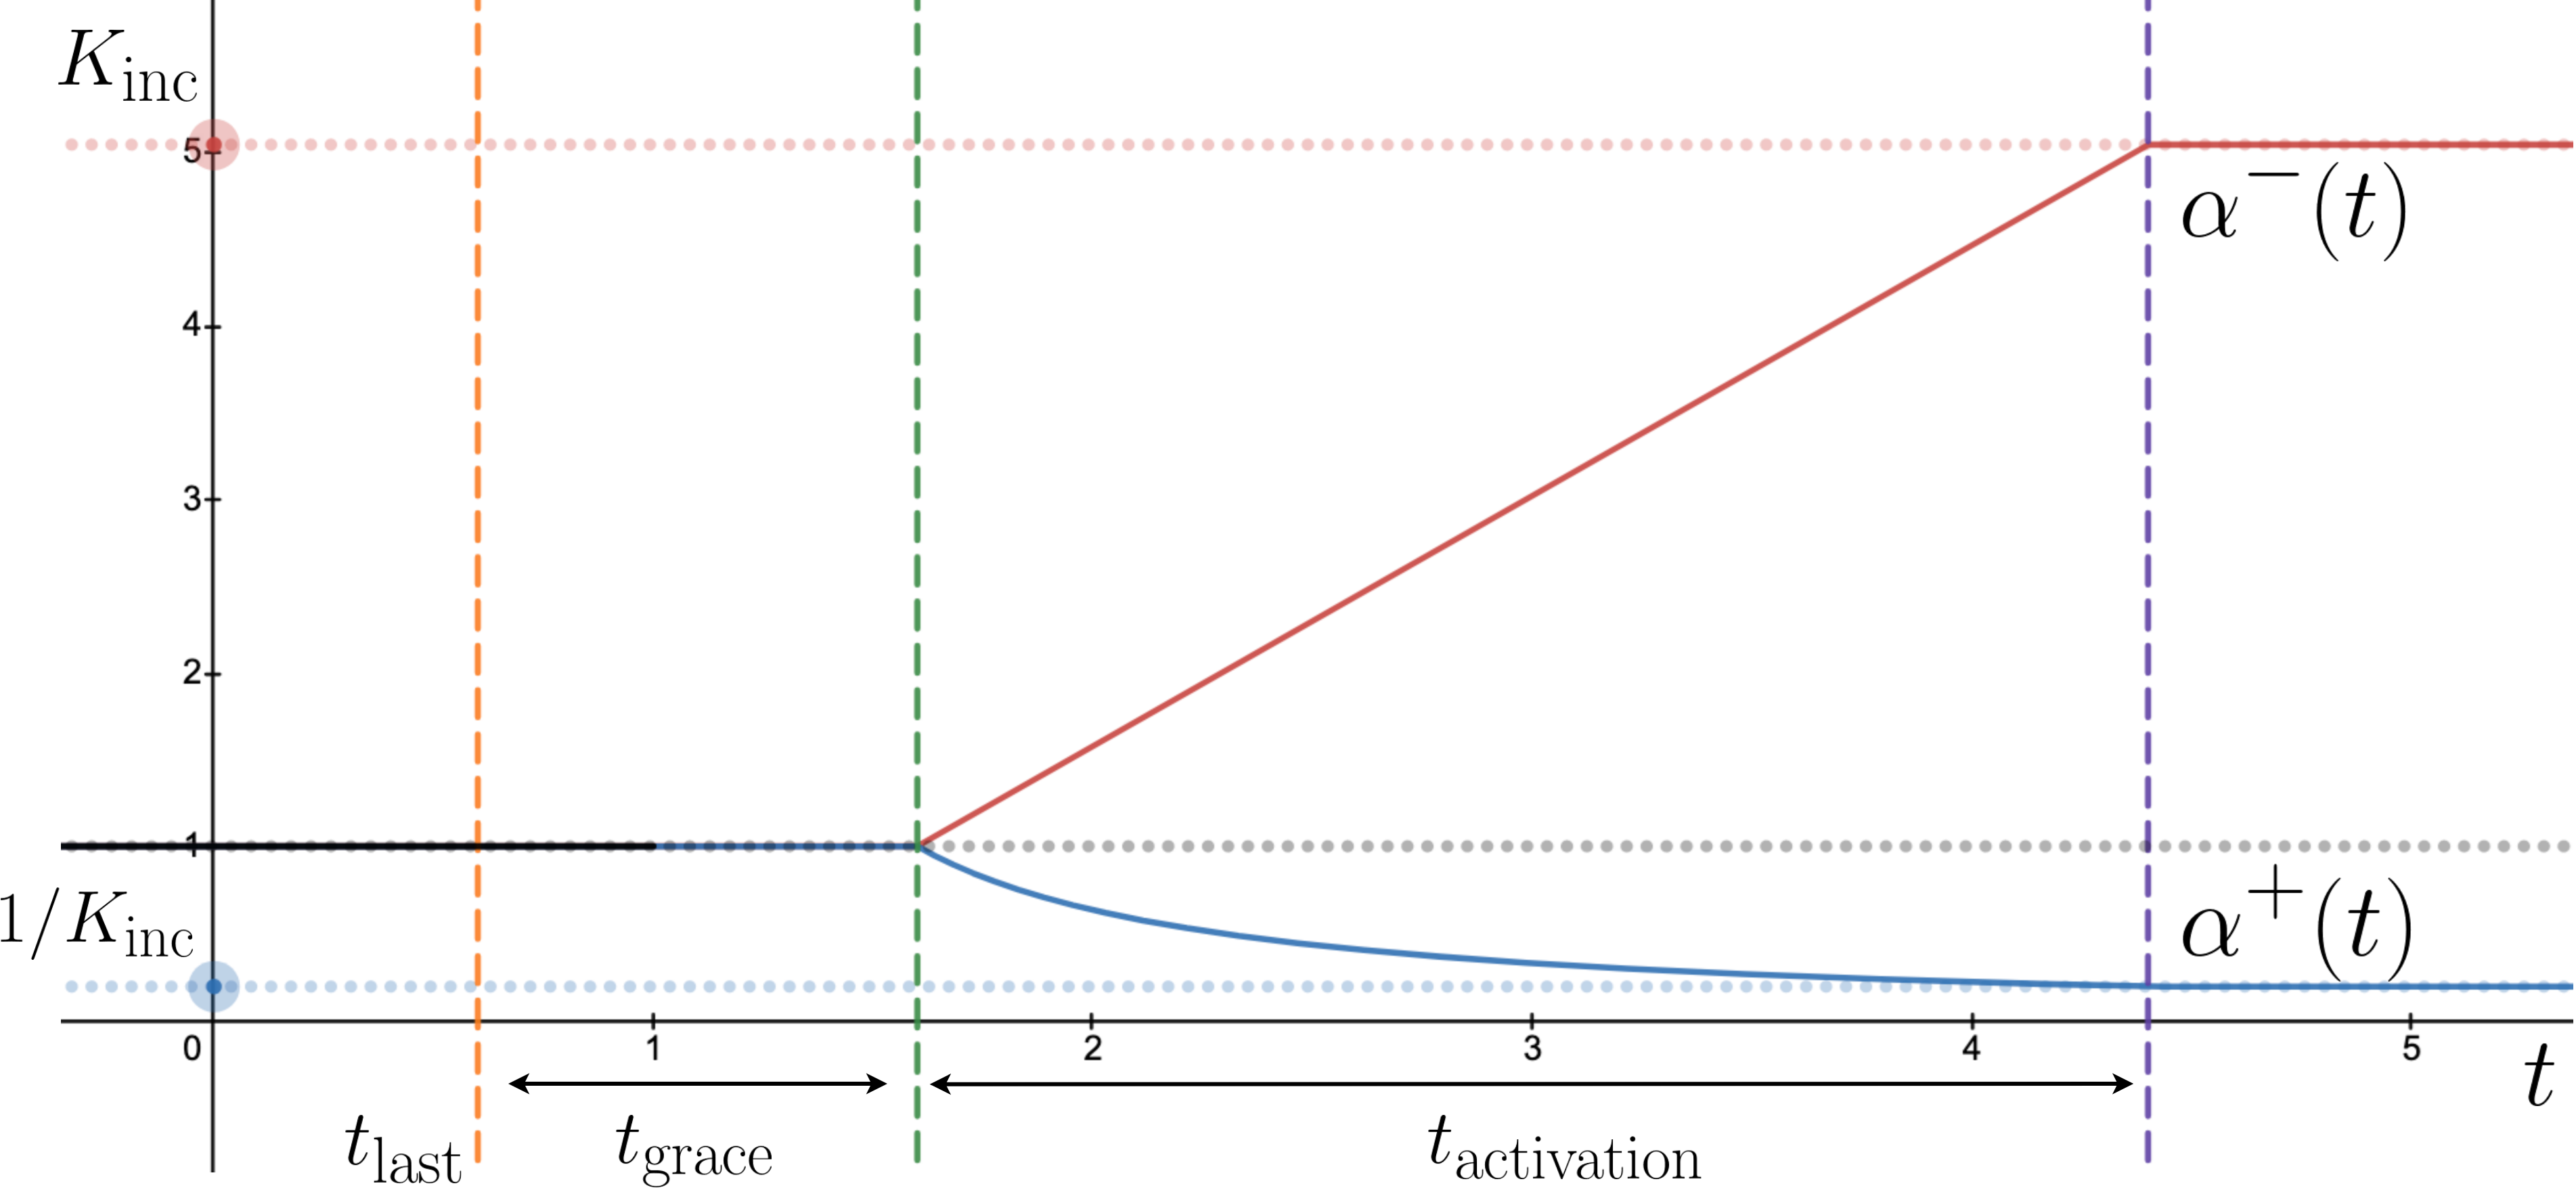
\includegraphics[width=0.9\linewidth]{fig/incentive_graph.png}
 \captionof{figure}{The graphs of $\alpha^+(t)$ (blue) and $\alpha^-(t)$ (red), which are multiplicative inverses of each other if $t^+_\textnormal{rel}(t)=t^-_\textnormal{rel}(t)$.}
\label{fig:incentive_multiplier_graphs}
\end{Figure}
\subsubsection{Multipliers}
% Parameters of incentives and averaging computations are $\{\alpha, \mu, t_\textnormal{init}, f_\textnormal{init}\}$.
Given the constant $K_\textnormal{inc}$  % does not make sense to initialize it as this is not a variable, we can just change all the constants to K_something later if desired.
% (initialized as $K_{\mathrm{RewardMultiplier}}$)
and the relative normalized time functions $t^+_\textnormal{rel}(t), t^-_\textnormal{rel}(t)$ established using state variables, we compute incentive multipliers $\alpha^+(t)$, $\alpha^-(t)$ as
\begin{align}
% \beta & \equiv  1 + (\alpha - 1)\cdot t_\textnormal{rel}(t, t_\textnormal{last},
%  t_\textnormal{avg})\\
% % \end{align}
% % \begin{align}
% \Gamma_\textnormal{inc}(t, t_\textnormal{last},
%  t_\textnormal{avg}) & \equiv
%  \begin{dcases}
%     \frac{1}{\beta}, &\text{if a \emph{proposal}} \\
%      \beta, &\text{if a \emph{proof}}
% \end{dcases}
\alpha^+(t) &= \nicefrac{1}{1 + (K_\textnormal{inc} - 1)\cdot t_\textnormal{rel}^+(t)}\\
\alpha^-(t) &= 1 + (K_\textnormal{inc} - 1)\cdot t_\textnormal{rel}^-(t).
\end{align}
% We initialize $t_\textnormal{last} \equiv 0$ , $t_\textnormal{ave} \equiv t_\textnormal{init}$ and $f_\textnormal{avg}\equiv f_\textnormal{init}$. $\alpha$ is the maximum incentive ratio. $\mu$ is the momentum parameter for the moving average (higher $\mu$ makes the effects of individual updates smaller). $t_\textnormal{init}$ is the initial time gap average before any transactions. $f_\textnormal{init}$ is the initial multiplier for slot based prices.
% At every new transaction at time $t$, we compute the following in sequence:
% \begin{align}
% \beta & \equiv  1 + (\alpha - 1)\cdot t_\textnormal{rel}(t, t_\textnormal{last},
%  t_\textnormal{avg})\\
% % \end{align}
% % \begin{align}
% \Gamma_\textnormal{inc}(t, t_\textnormal{last},
%  t_\textnormal{avg}) & \equiv
%  \begin{dcases}
%     \frac{1}{\beta}, &\text{if a \emph{proposal}} \\
%      \beta, &\text{if a \emph{proof}}
% \end{dcases}
% \end{align}
% As shown by the figure below, the proposing fee can be reduced to $\nicefrac{f_\textnormal{b}}{\alpha}$, and the proving reward can be amplified up to $f_\textnormal{b} \cdot \alpha$.
As shown in Figure \ref{fig:incentive_multiplier_graphs}, the incentive multiplier for proof rewards, $\alpha^-(t)$, cannot exceed $K_\textnormal{inc}$ and the incentive multiplier for proposal fees, $\alpha^+(t)$, cannot be less than $\nicefrac{1}{K_\textnormal{inc}}$.

\subsection{Slot-availability Multipliers}
\label{sec:slot_availability_multipliers}
% Removing this part for now, as it is not quite there (it introduces new variables not well defined and are not used directly). I will consider this reasoning later on and see if it can be added on.
% The expected number of unverified blocks is $\nicefrac{t^\textnormal{p}_\textnormal{ave}}{t^\textnormal{b}_\textnormal{ave}}$, where $t^\textnormal{b}_\textnormal{ave}$ is the average block proposal time and $t^\textnormal{p}_\textnormal{ave}$ is the average proof delay.
% When the number of unverified blocks is smaller than expected, the proposing fee shall be reduced to encourage block proposals; otherwise the proof reward shall be increased to encourage prover engagement.
% Instead of relying on the comparison with $\nicefrac{t^\textnormal{p}_\textnormal{ave}}{t^\textnormal{b}_\textnormal{ave}}$, this can be accomplished using the \emph{constant-product} pricing mechanism as used by Uniswap V1.
Slot-availability multipliers are computed solely from the current number of unverified blocks $n$ and they are independent of time given a particular state.

These multipliers capture the idea of offering the lowest fees and rewards when there are only a few unverified blocks and a surplus of available slots, $n_\textnormal{slots}-n$. In this case, parallel proof computation can accommodate many proposers, which leads to low competition and consequently lower fees. Further, there is a shortage of unverified blocks to prove, which means that provers must compete with each other to get the rewards (which allows lower rewards).

In the opposite case, the level of competition for proposers and provers are reversed when there are many unverified blocks. As the number of available slots, $n_\textnormal{slots}-n$, decrease, competition for the remaining slots increase for proposers, which leads to higher fees. Further, since there are many unverified blocks, competition for provers is low, which results in higher rewards.

% In the opposite case of many unverified blocks, fees are higher as new proposers must compete to get the last few available slots. Similarly, the rewards are higher because there are plenty of unverified blocks to go around for provers.

Therefore, fees and rewards increase as the number of unverified blocks grow, through multipliers $\beta^+(n)$ and $\beta^-(n)$ respectively, which are governed by a
% \emph{constant-product}
pricing mechanism used in Uniswap V1, described below.

Given a smoothing constant $K_\textnormal{slot} \geq 1$ that determines how slowly the slot-availability multipliers increase as $n$ grows,
% another constant, $\Phi$, is computed from $n_\textnormal{slots}$ and $\lambda$.
% \begin{align}
%     % \Phi \equiv \underbrace{(n_\textnormal{slots} + \lambda - 1)}_{k(t=0)} \cdot \underbrace{(n_\textnormal{slots} + \lambda)}_{n_\textnormal{slots}-n(t=0) + \lambda}\\
%     \Phi \equiv (n_\textnormal{slots}- 1 + \lambda ) \cdot (n_\textnormal{slots} + \lambda)
% \end{align}
% This invariant remains the same across all time, as the number of available slots $n(t)$ changes by $m$ blocks due to successful proposals and proofs:
% \begin{align}
%     \Phi(t) \equiv k(t, m) \cdot (n(t) + \lambda + m) \equiv \Phi
% \end{align}
% This requires that $k(t, m) \equiv \nicefrac{\Phi}{n(t) + \lambda} + m$. Therefore, $k(t, m)$ at any given time follows an inverse law with respect to available slots $n(t)$.
% At any given time point $t$, we can update the fee or reward $f(t)$ as:
% \pagebreak
we define $\beta^+(n): \{n\in \mathbb{Z} \hspace{0.02in}|\hspace{0.02in}  0 \leq n < n_\textnormal{slots} \}\rightarrow \mathbb{R}^+$ and $\beta^-(n): \{n\in \mathbb{Z} \hspace{0.02in}|\hspace{0.02in}  0 < n \leq n_\textnormal{slots} \}\rightarrow \mathbb{R}^+$ as,

% \begin{align}
% \beta_f(n) &= \frac{\Phi}{(n_\textnormal{slots}-n-1 + \lambda)\cdot (n_\textnormal{slots}-n + \lambda)}\\
% \beta_r(n) &= \frac{\Phi}{(n_\textnormal{slots}-n + 1 + \lambda)\cdot (n_\textnormal{slots}-n + \lambda)}
% \end{align}

\begin{align}
n'_\textnormal{slots} &= n_\textnormal{slots} + K_\textnormal{slot} \\
\beta^+(n) &= \frac{(n'_\textnormal{slots}- 1) \cdot n'_\textnormal{slots}}{(n'_\textnormal{slots}-n-1)\cdot (n'_\textnormal{slots}-n)}\\
\beta^-(n) &= \frac{(n'_\textnormal{slots}- 1 ) \cdot n'_\textnormal{slots}}{(n'_\textnormal{slots}-n + 1)\cdot (n'_\textnormal{slots}-n)}.
\end{align}
% (n_\textnormal{slots}- 1 + \lambda ) \cdot (n_\textnormal{slots} + \lambda)
% \begin{align}
% m & \equiv &
% \begin{dcases}
%    -1, & \text{if a \emph{proposal}} \\
%     1, & \text{if a \emph{proof}} \\
% \end{dcases}\\
% f^*(t) & \equiv & f(t) \cdot  \left\lvert k(t, 0) - k(t, m)\right\lvert \\
% \nonumber& \equiv & f(t) \cdot \left\lvert \frac{\Phi}{n(t) + \lambda}-\frac{\Phi}{n(t) + \lambda + m}\right\lvert \\
% \nonumber & \equiv & f(t) \cdot  \frac{\Phi}{(n(t) + \lambda + m)\cdot (n(t) + \lambda)}
% \end{align}
It is easy to see that for $n=0$, which corresponds to the case of not having any unverified blocks, the multiplier for fees is
% \begin{align}
% \beta_f(0) &= \frac{\Phi}{(n_\textnormal{slots}-1 + \lambda)\cdot (n_\textnormal{slots} + \lambda)}=1
% \end{align}
\begin{align}
\beta^+(0) &= \frac{(n'_\textnormal{slots}- 1 ) \cdot n'_\textnormal{slots}
}{(n'_\textnormal{slots}-1)\cdot n'_\textnormal{slots}}=1.
\end{align}
% (n_\textnormal{slots}- 1 + \lambda ) \cdot (n_\textnormal{slots} + \lambda)
% simply from the definition of $\Phi$.
In this case, the overall fee simplifies to
\begin{align}
f(t) = f_\textnormal{base} \cdot \alpha^+(t).
\end{align}

Further, if $n = n_\textnormal{slots}-1$ (only one slot is available),  the multiplier for fees takes its maximum value,
\begin{align}
\beta^+(n_\textnormal{slots}-1)
% &= \frac{\Phi}{(\lambda)\cdot (1 + \lambda)} \\
% \nonumber
&=
\frac{(n_\textnormal{slots}- 1 + K_\textnormal{slot} ) \cdot (n_\textnormal{slots} + K_\textnormal{slot})}{K_\textnormal{slot}\cdot (1 + K_\textnormal{slot})}.
\end{align}

Finally, we note that for all valid inputs $\{n\in \mathbb{Z} \hspace{0.02in}|\hspace{0.02in}  0 \leq n < n_\textnormal{slots} \}$,
\begin{align}
    \beta^-(n+1) = \beta^+(n)
\end{align}
which ensures that the multiplier of the reward for a proven block equals the multiplier for its fee when it was proposed.

% \begin{align}
% f^*(t)  & \equiv & f(t) \cdot \frac{\Phi}{\lambda\cdot (1+\lambda)} \\
% \nonumber & \equiv & f(t) \cdot \frac{(n_\textnormal{max} + \lambda - 1) \cdot (n_\textnormal{max} + \lambda)}{\lambda\cdot (1+\lambda)}
% \end{align}

% If we hold $f(t)$ constant, the ratio between the last and the first slot's proposal fee is,
% \begin{align}
% % \frac{f(1)}{f(n_{\textnormal{max}})} =
% R  \equiv \frac{(n_\textnormal{max} + \lambda - 1) \cdot (n_\textnormal{max} + \lambda)}{\lambda\cdot (1+\lambda)}.
% \end{align}

\begin{Figure}
 \centering
 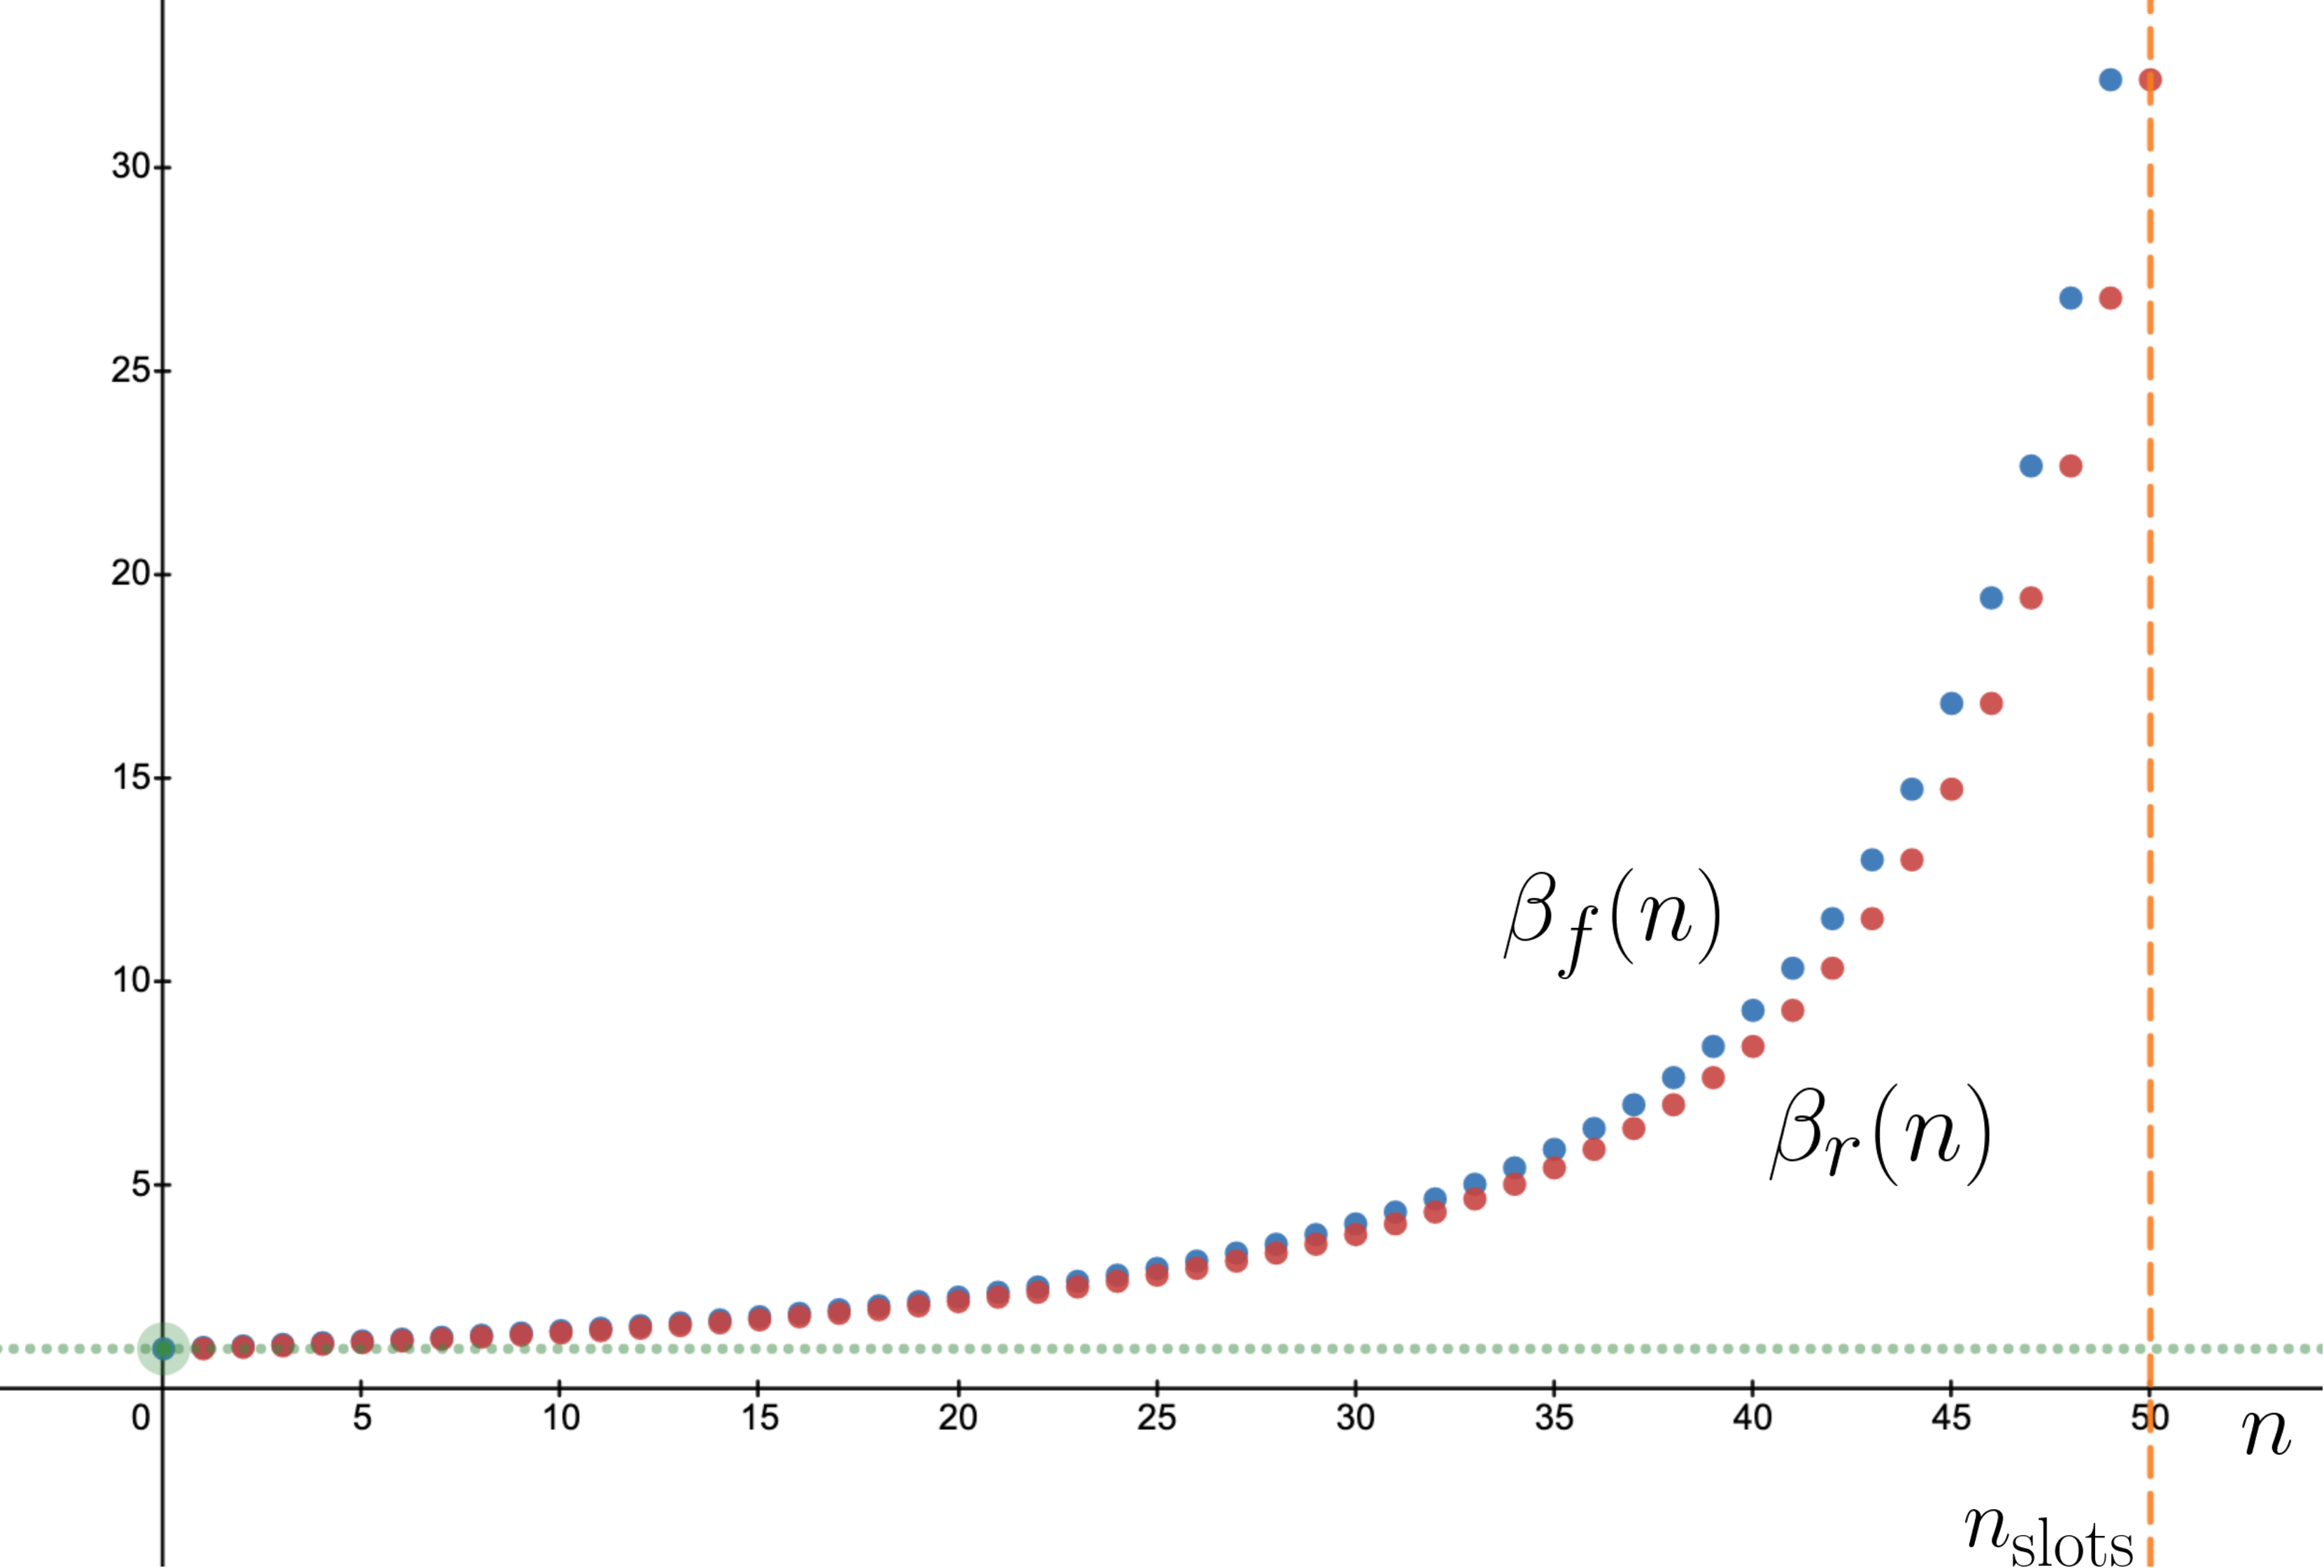
\includegraphics[width=0.8\linewidth]{fig/lambda10.png}
 \captionof{figure}{Progression of the multiplier for fees $\beta^+(n)$ (blue) and the multiplier for rewards $\beta^-(n)$ (red), when $n_{\textnormal{slots}}=50$ and $K_\textnormal{slot}=10$. The maximum value of the multiplier is $\frac{(n_\textnormal{slots} - 1 + K_\textnormal{slot} ) \cdot (n_\textnormal{slots} + K_\textnormal{slot})}{K_\textnormal{slot}\cdot (1+K_\textnormal{slot})}=32.182$.}
 \label{fig:f_slot_lambda1}
\end{Figure}

Finally, in Figures \ref{fig:f_slot_lambda1} and \ref{fig:f_slot_lambda50}, we demonstrate that the smoothing term $K_\textnormal{slot}$ can be increased to attenuate the maximum value of slot-availability multipliers.

\begin{Figure}
 \centering
 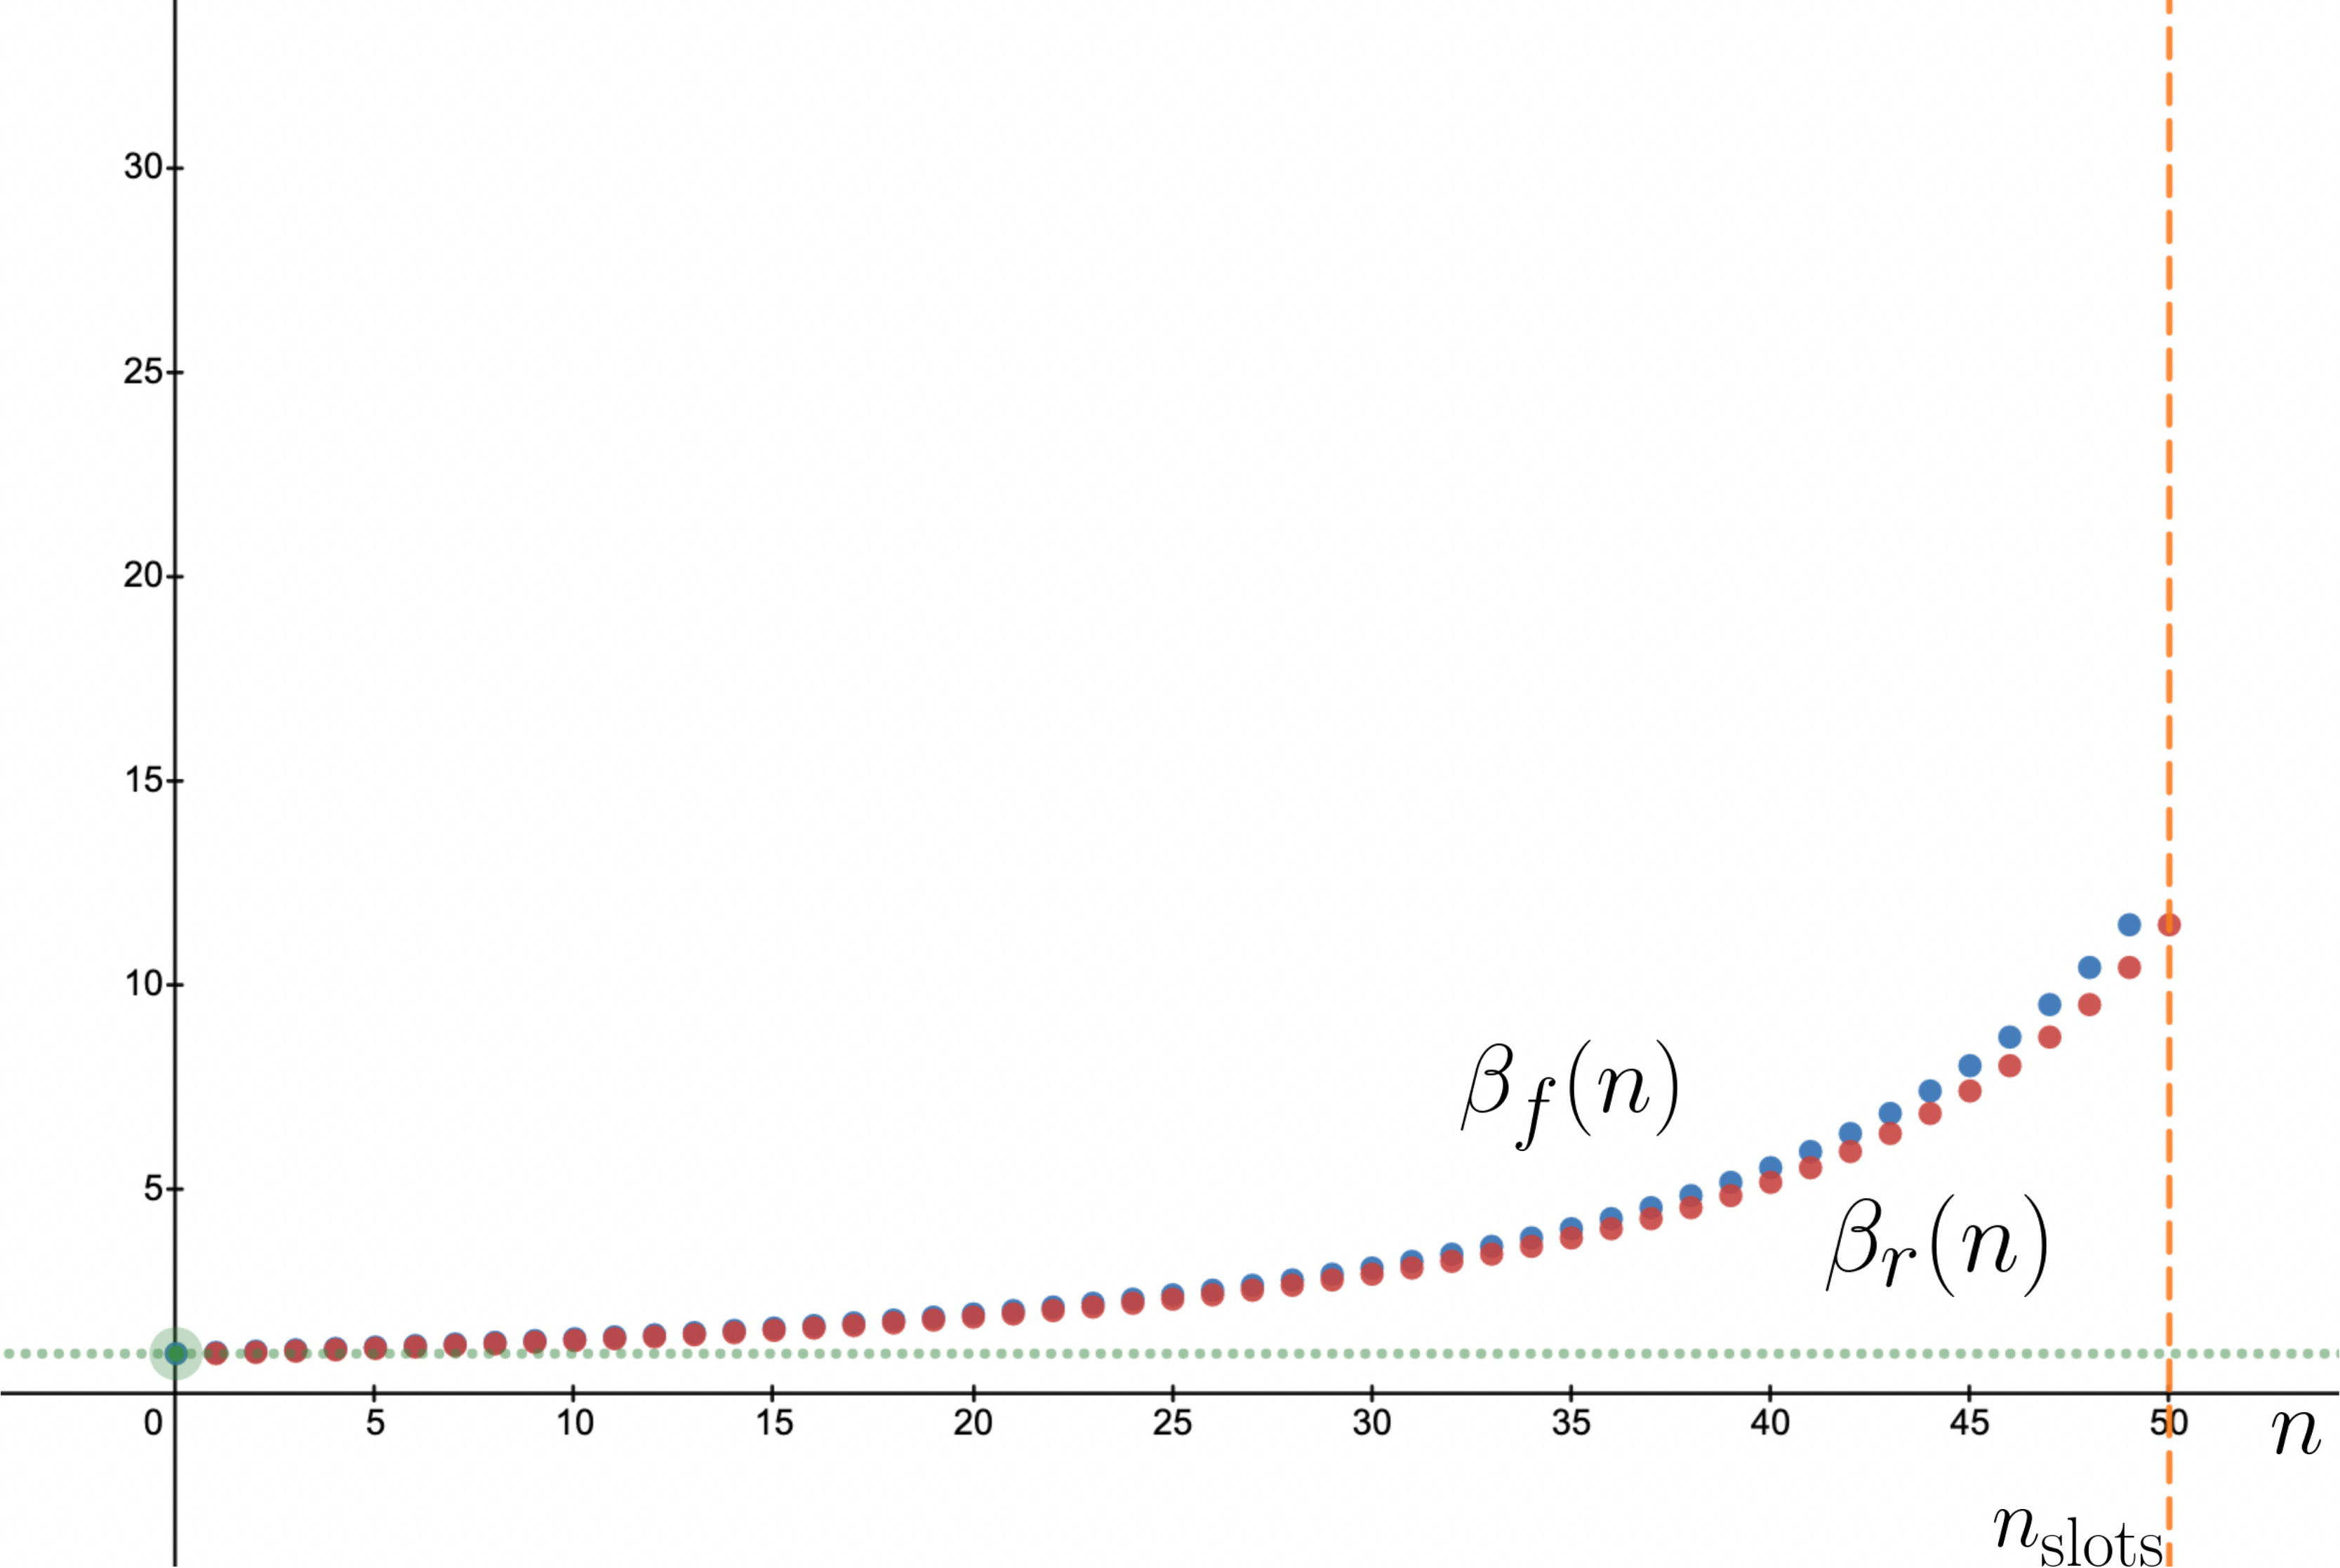
\includegraphics[width=0.8\linewidth]{fig/lambda20.png}
 \captionof{figure}{Progression of the multiplier for fees $\beta^+(n)$ (blue) and the multiplier for rewards $\beta^-(n)$ (red), when $n_{\textnormal{slots}}=50$ and $K_\textnormal{slot}=20$. The maximum value of the multiplier is $\frac{(n_\textnormal{slots} - 1 + K_\textnormal{slot} ) \cdot (n_\textnormal{slots} + K_\textnormal{slot})}{K_\textnormal{slot}\cdot (1+K_\textnormal{slot})}=11.5$.}
 \label{fig:f_slot_lambda50}

\end{Figure}

\subsection{Bootstrap Discount Multipliers}\label{sec:bootstrapping}
Unlike block provers, proposers are directly affected by the number of active L2 users, as well as ETH fees they need to pay to the L1-layer validators. This makes them vulnerable at the initial stages of the protocol when there are not many L2 users engaging it with their transactions, which makes it hard for proposers to create larger and more profitable blocks with many transactions in them.

\begin{Figure}
 \centering
 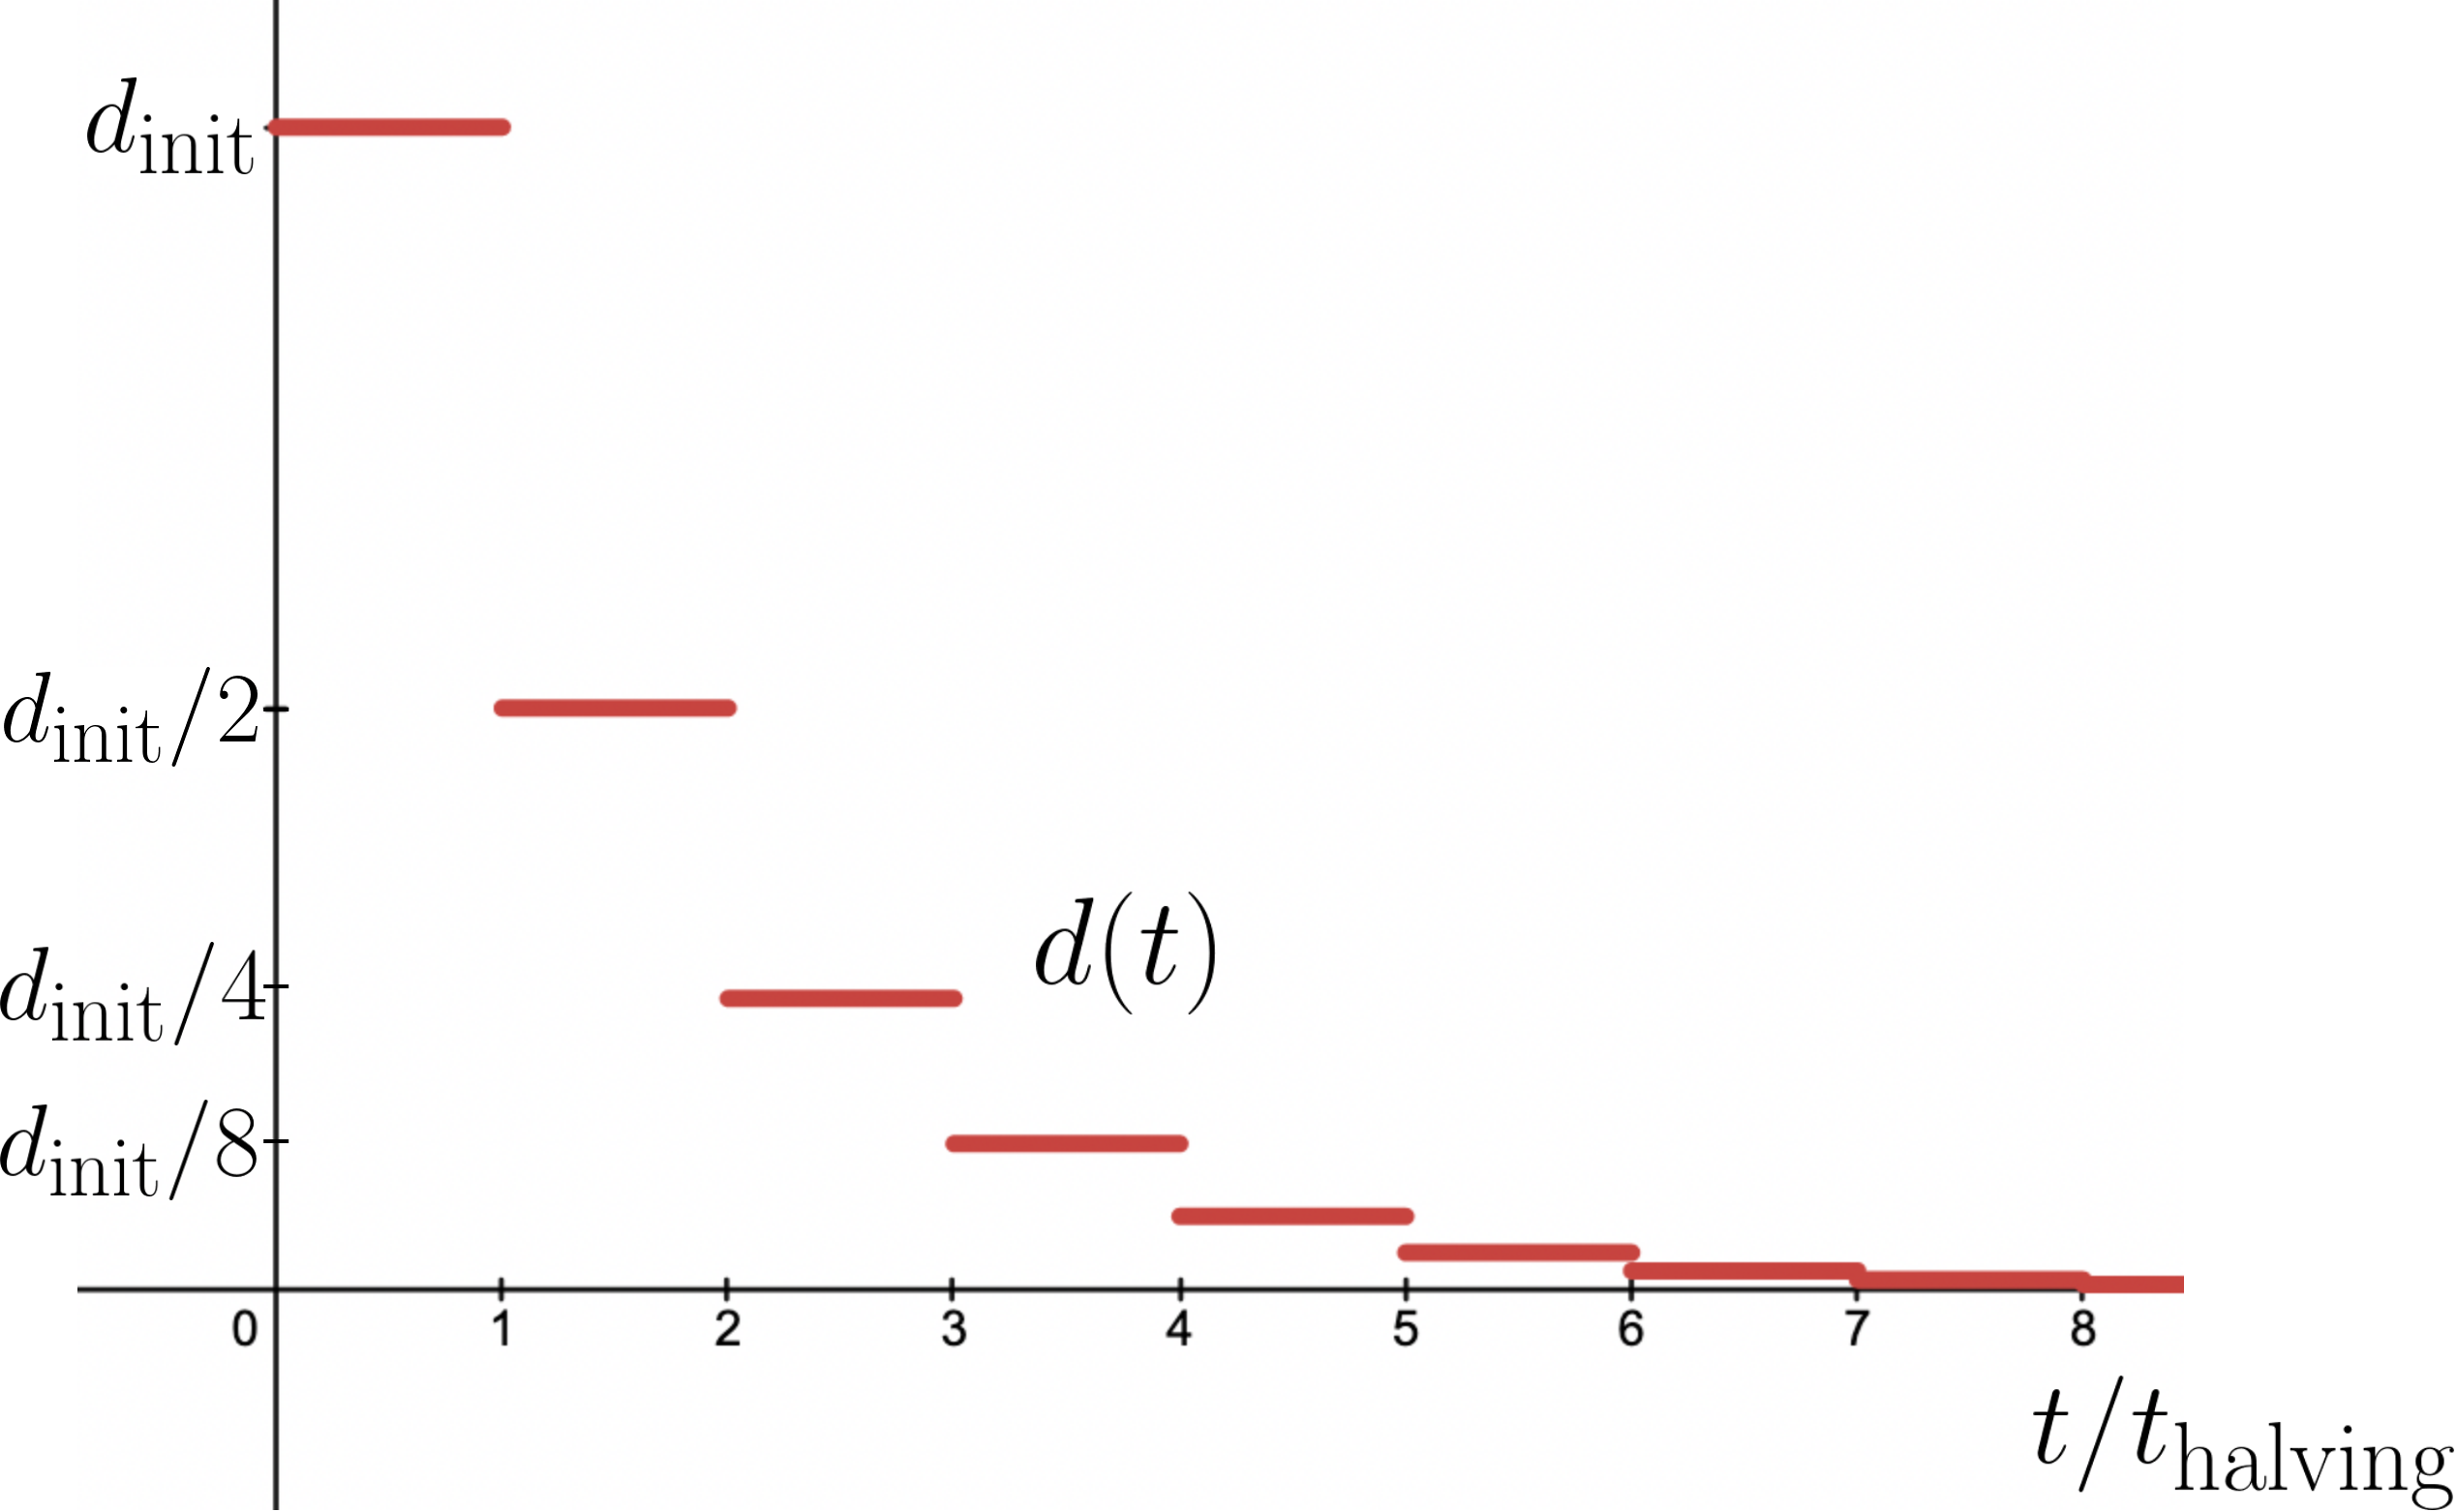
\includegraphics[width=0.8\linewidth]{fig/discount_func.png}
 \captionof{figure}{Graph of discount function $d(t)$.}
 \label{fig:discount}
\end{Figure}

Given an initial discount rate constant $K_\textnormal{disc} \in (0, 1]$ and a halving period constant $K_\textnormal{Halving} > 0$, we can compute a discount function $d(t)$ and a discount multiplier for fees $\gamma^+(t)$ as functions of time:

\begin{align}
d(t) &= K_\textnormal{disc}\cdot (\nicefrac{1}{2})^{\lfloor \nicefrac{t}{K_\textnormal{Halving}}\rfloor}
\\
\gamma^+(t)  &= 1-d(t).
\end{align}

As time passes, this multiplier approaches $1$, which means that its effects diminish over time.

The discount multiplier is applied to the overall proposal fee computation as follows:
%
% During the bootstrapping period after the network goes live, block proposers may not be able to collect enough transactions to justify their proposing fees. Therefore, a dedicated pool of TKO token, $B = K_{\mathrm{BootstrapReward}}$, is set up to reward early block proposers over a period $T = K_{\mathrm{BootstrapPeriod}}$ so they are willing to keep proposing smaller blocks.
%
% For each block, the bootstrapping reward $r(t)$ is calculated as


% \begin{eqnarray}
% \\
% \nonumber r(t) \equiv
%  \begin{dcases}
%     \frac{(T - t_\textnormal{last})^2 - (T - t)^2}{T^2} \cdot B, &\text{if} \quad t < T \\
%     0, &\text{otherwise}
% \end{dcases}
% \end{eqnarray}

% The larger the gaps between $t_\textnormal{last}$ and $t$ is, the larger the bootstrapping reward will be.

\begin{align}
f(t) = f_\textnormal{base} \cdot \alpha^+(t) \cdot \beta^+(n) \cdot \gamma^+(t)
\end{align}

Bootstrapping support is applicable only to proposer fees in order to safeguard the normal market order conditions between proposers and provers.

\subsection{State Update}
Given a momentum constant $ 0\leq \mu \leq 1$, we update state variables in the following order after each successful block proposal submitted at time $t$:
\begin{gather}
    n \equiv n + 1\\
f_\textnormal{base} \equiv
\frac{\mu-1}{\mu} \cdot f_\textnormal{base} + \frac{1}{\mu} \cdot f_\textnormal{base}\cdot \alpha^+(t)
%  \begin{dcases}
%      \frac{\mu-1}{\mu} \cdot f_\textnormal{base} + \frac{1}{\mu} \cdot f_\textnormal{base}\cdot \alpha^+(t), &\text{if a \emph{proposal}} \\
%       \frac{\mu-1}{\mu} \cdot f_\textnormal{base} + \frac{1}{\mu} \cdot f_\textnormal{base} \cdot \alpha^-(t), &\text{if a \emph{proof}}
% \end{dcases}
\\
t^+_\textnormal{ave} \equiv
\frac{\mu-1}{\mu} \cdot t^+_\textnormal{ave} + \frac{1}{\mu} \cdot (t-t^+_\textnormal{last})
\\
% t^-_\textnormal{ave} \equiv
% \frac{\mu-1}{\mu} \cdot t^-_\textnormal{ave} + \frac{1}{\mu} \cdot (t-t^-_\textnormal{last})
% \\
t^+_\textnormal{last} \equiv t
% \\
% t^-_\textnormal{last} \equiv t
\end{gather}

Similarly, once a proof submitted at time $t$ is validated, we update the state variables in the following order:
\begin{gather}
    n \equiv n - 1
%  \begin{dcases}
%      n - 1, &\text{if a \emph{proposal}} \\
%       n + 1, &\text{if a \emph{proof}}
% \end{dcases}
\\
f_\textnormal{base} \equiv
\frac{\mu-1}{\mu} \cdot f_\textnormal{base} + \frac{1}{\mu} \cdot f_\textnormal{base} \cdot \alpha^-(t)
%  \begin{dcases}
%      \frac{\mu-1}{\mu} \cdot f_\textnormal{base} + \frac{1}{\mu} \cdot f_\textnormal{base}\cdot \alpha^+(t), &\text{if a \emph{proposal}} \\
%       \frac{\mu-1}{\mu} \cdot f_\textnormal{base} + \frac{1}{\mu} \cdot f_\textnormal{base} \cdot \alpha^-(t), &\text{if a \emph{proof}}
% \end{dcases}
\\
t^-_\textnormal{ave} \equiv
\frac{\mu-1}{\mu} \cdot t^-_\textnormal{ave} + \frac{1}{\mu} \cdot (t-t^-_\textnormal{last})
\\
t^-_\textnormal{last} \equiv t
\end{gather}

% After computing $f_\textnormal{avg}(t)$ for the current transaction, we update $f_\textnormal{avg}$, $t_\textnormal{ave}$ and $t_\textnormal{last}$:
% \begin{eqnarray}
% f_\textnormal{avg} & \equiv & \frac{\mu-1}{\mu} \cdot f_\textnormal{avg} + \frac{1}{\mu} \cdot f(t)\\
% t_\textnormal{ave} & \equiv & \frac{\mu-1}{\mu} \cdot t_\textnormal{ave} + \frac{1}{\mu} \cdot (t-t_\textnormal{last})\\
% t_\textnormal{last} & \equiv & t_\textnormal{new}
% \end{eqnarray}

The state update for $f_\textnormal{base}$ incorporates time-based incentives into a more permanent effect using a moving average. If proposals utilize incentives more actively compared to proofs, $f_\textnormal{base}$ decreases for future transactions. If proofs utilize incentives more actively, $f_\textnormal{base}$ increases over time.


% This step incorporates incentives into a more permanent change to the overall pricing through $f_\textnormal{avg}$. If proposals utilize incentives more actively compared to proofs, $f_\textnormal{avg}$ reduces for future transactions. If proofs utilize them more actively, $f_\textnormal{avg}$ increases over time.

\label{sec:priceStateUpdate}

